\section{理想滤波器}

本节介绍理想滤波器的概念,随后讨论理想低通的可能性。

本节要点:
\begin{itemize}
    \item 理解4类理想滤波器;
    \item 从因果律理解低通滤波器。
\end{itemize}

%============================================================
\subsection{理想滤波器的幅频和相频要求}

幅频上考察,理想滤波器分为:
\begin{itemize}
    \item {\bf 低通}(lowpass),$\left| H\left( \omega \right) \right|=1,\omega \in \left[ -B,B \right] $,并称$B$为{\bf 滤波器带宽};
    \item {\bf 高通}(highpass),$\left| H\left( \omega \right) \right|=1,\omega \notin \left[ -B,B \right] $;
    \item {\bf 带通}(bandpass),$\left| H\left( \omega \right) \right|=1,\omega \in \left[ -B_1,B_2 \right] $,并称$B_2-B_1$为{\bf 滤波器带宽};
    \item {\bf 带阻}(bandstop),$\left| H\left( \omega \right) \right|=1,\omega \notin \left[ -B_1,B_2 \right] $。
\end{itemize}
理想滤波器对于通带没有任何衰减,对于禁带则完全衰减。

相频上,理想滤波器必须满足频率的线性性:
\[
\angle H\left( \omega \right) =-a\omega \qquad a\geqslant 0
\]
为满足因果律,必须$a\geqslant 0$,使得输出相对输入是延时的,才能使任何频率的正弦波没有频率扭曲。
\[
y\left( t \right) =A\left| H\left( \omega \right) \right|\cos \left( \omega _0t-a\omega _0 \right) =A\left| H\left( \omega \right) \right|\cos \left[ \omega _0\left( t-a \right) \right]
\]
\begin{figure}[h]
\centering
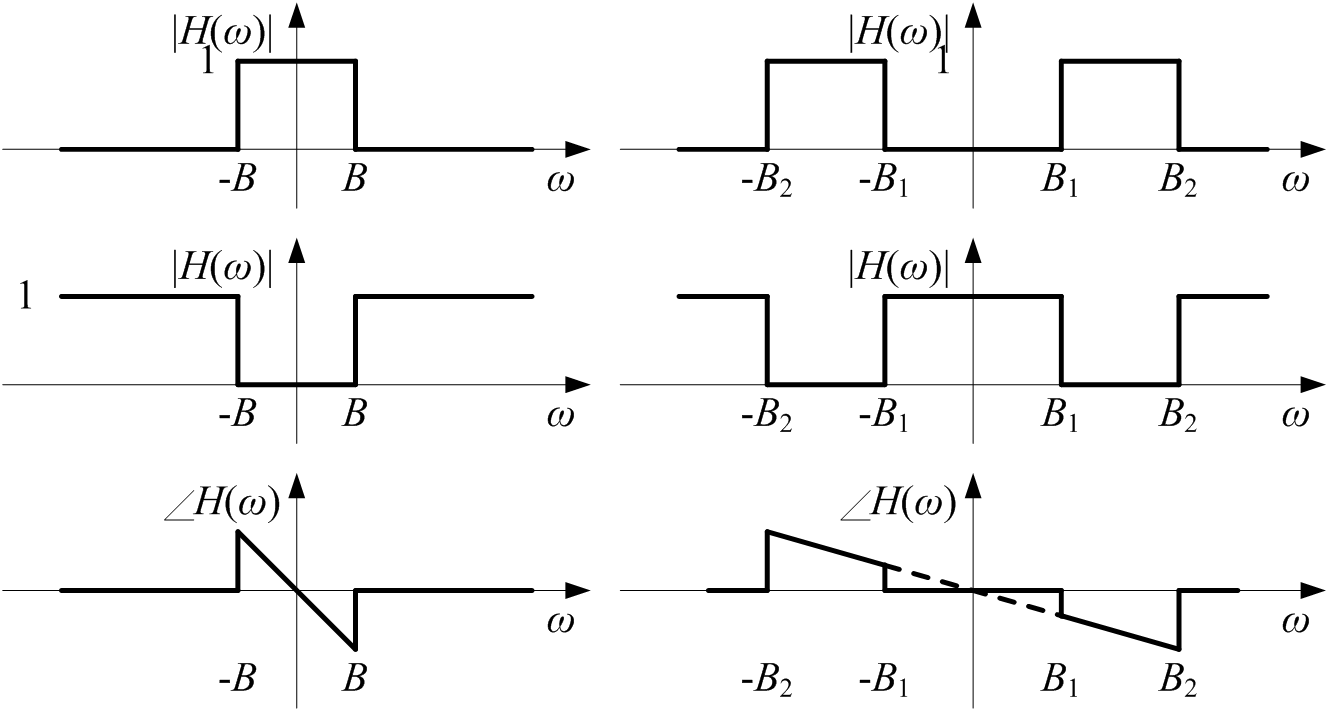
\includegraphics[height=6cm]{5.2.1-1.png}
\end{figure}

%============================================================
\subsection{理想低通滤波器的可能性}

理想的“全通”的频率响应应符合大小无衰减且相位线性,于是有:
\begin{align*}
&\because \begin{cases}
	\left| H\left( \omega \right) \right|=1\\
	\angle H\left( \omega \right) =-a\omega\\
\end{cases} \\
&\therefore H\left( \omega \right) =e^{ia\omega}
\end{align*}
则理想低通相当于全通被方波函数包络:
\[
H\left( \omega \right) =p_{2B}\left( \omega \right) \cdot e^{ia\omega}
\]
这是理想低通的频率响应。
根据傅里叶变换性质,系统的冲激响应:
\[
h\left( t \right) =\frac{B}{\pi}\mathrm{sinc}\frac{B\left( t-a \right)}{\pi}
\]
\begin{itemize}
    \item $B$:系统带宽;
    \item $a$:系统延时。
\end{itemize}
由于冲激响应在$t<0$都会有值,相当于作为输入的冲激还没有进系统,系统就有输出。
这种系统违反了因果律,所以理想低通是不存在的。




